\subsection*{Visitor Pattern}\label{subs:visit}
The visitor pattern is not only used to traverse the parse tree provided by ANTLR, but also the \acrfull{ast}.
The visitor pattern is implemented throughout the compiler, to create the \acrfull{ast} from the parse tree, for traversing the \acrfull{ast} for pretty printing, as well as for filling the symbol table, type and scope checking, and also for code generation.
As such the visitor pattern defines the structure of the compiler, and thus understanding what is gained from using this pattern is important.
The visitor pattern is one of the design patterns by the Gang of Four, authors of ``Design Patterns: Elements of Reusable Object-Oriented Software''.
Its description says ``The visitor pattern is a design pattern that separates a set of structured data from the functionality that may be performed upon it.''. \citep{GOF}

The pattern is a behavioral pattern i.e. it defines how communication between classes and entities are handled.
In the tree walk for the parse tree, the visitor should convert the parse tree into a \acrfull{ast}.
This entails that each different node in the parse tree must be visited to find the information needed to create the \acrfull{ast}.

Through use of the visitor pattern the functionality is separated from the classes they are performed upon. 
Instead the functionality is on a visitor class implementing the visitor interface, which means different visitors can be made, which all do different computations while traversing the tree.
Each class in the tree have an \texttt{accept} method that allows them to call the visitor in question with itself as an argument.
This allows the ability of adding new operations without changing the original data structure, and also without changing other visitors, an invaluable feature when doing iterative development.
Another benefit is that a single visitor object is used to visit all the classes in the tree.
This visitor can therefore maintain a state between calls to individual data objects, which can be used to save information in an outer scope from the different visit calls.
\myref{image:visitor} shows a UML diagram of the visitor pattern.
This diagram is from a C\# representation, and while the idea is the same the exact implementation is not identical to the one used in the compiler for GAMBLE.
The most important things to take note of are the classes ``ConcreteElement'' and ``ConcreteVisitor''.
The ``ConcreteElement'' represent the different kinds of nodes in a given tree.
The ``ConcreteVisitor'' represent the different kind of visitors implemented, this being one for AST, parse tree, symbol table filling, scope and type checking, code generation and pretty print, all these implements an interface that contains visit methods for each ``ConcreteElement''.

\begin{figure}[h!]
\centering
 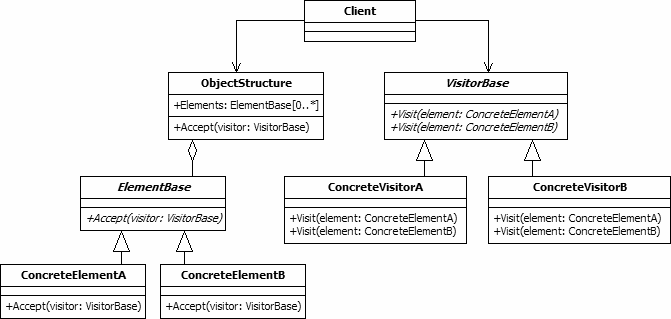
\includegraphics[width=1\textwidth]{figures/VisitorPattern.png} % trim=4.85cm 15cm 0.85cm 1cm
\caption{A UML diagram for the implementation of the visitor pattern in a C\# environment}\label{image:visitor}
\vspace{-15pt}
\end{figure}


